\documentclass[a4paper,12pt]{article} 

%%%%%%%%%%%%%%%%%%%%%%%%%%%%%%%%%%%%%%%%%%%%%%%%%%%%%%%%%%%%%%%%%%%%%%%%%%%%
\usepackage[utf8]{inputenc}
\usepackage[spanish]{babel}
\usepackage{amsmath}
\usepackage{amsfonts}
\usepackage{amssymb} 
\usepackage{graphicx} 
\usepackage{hyperref} 
\usepackage{wrapfig}
\usepackage{enumitem}
\usepackage{blindtext}
\usepackage{fancyhdr}
\usepackage{float}
\usepackage{eurosym}
\usepackage{color}
\usepackage{titling}
\usepackage{amssymb, amsmath, amsbsy} % simbolitos
 \usepackage{upgreek} % para poner letras griegas sin cursiva
 \usepackage{cancel} % para tachar
 \usepackage{mathdots} % para el comando \iddots
 \usepackage{mathrsfs} % para formato de letra
\usepackage{stackrel} % para el comando \stackbin
\usepackage{lipsum}
\usepackage{tocbibind}
\usepackage[T1]{fontenc}
\usepackage[left=3cm,right=3cm,top=3cm,bottom=4cm]{geometry}
\pagestyle{fancy}
%%%%%%%%%%%%%%%%%%%%%% CABECERAS %%%%%%%%%%%%%%%%%%%%%%%%%%%%%%%%%%%%%%%%%%%
\newcommand{\hsp}{\hspace{20pt}}
\newcommand{\HRule}{\rule{\linewidth}{0.5mm}}
\headheight=50pt
\newcommand{\vacio}{\textcolor{white}{holacaracola}}
%%% NUMERACION DE ECUACIONES
\renewcommand{\theequation}{\thesection.\arabic{equation}}
% COLOR AZUL PARA TEXTOS EN PORTADA
\definecolor{azulportada}{rgb}{0.16, 0.32, 0.75}
% Azul para textos de headings
\definecolor{azulinterior}{rgb}{0.0, 0.2, 0.6}

%%%%%%%%%%%%%%%%%%% DATOS DEL PROYECTO %%%%%%%%%%%%%%%%%%%%%%%%%%%%%%%%%%%%%
\title{Atividad 8}
\author{}
\newcommand{\director}{Carlos Lizárraga Celaya}

\begin{document}
\begin{titlepage}
\begin{center}
\vspace{1cm}

\includegraphics[width=5.5cm]{unison-logo.png}
\\[0.5cm]
{\fontfamily{phv}\fontsize{24}{6}\selectfont{UNIVERSIDAD DE SONORA}}\\
[1em]
{\fontfamily{phv}\fontsize{16}{5}\selectfont{DEPARTAMENTO DE FÍSICA}}\\
[4em]
\textcolor{azulportada}
{\fontfamily{phv}\fontsize{30}{5}\selectfont{\textsc{\thetitle}}}\\
% Autor del trabajo de investigación
[1cm]
{\fontfamily{phv}\fontsize{16}{5}\selectfont{Alumno:}}\\
[0.2cm]
%Equipo sfdsfshkfhsfhsjfs
{\fontfamily{phv}\fontsize{14}{5}\selectfont{Luis Alfonso Torres Flores}}\\
[1cm]
%{\Huge\textbf{\thetitle}}\\
{\fontfamily{phv}\fontsize{16}{5}\selectfont{Profesor}}\\
[0.2cm]
{\fontfamily{phv}\fontsize{16}{5}\selectfont{\director}}\\
[4.5cm]
{\fontfamily{phv}\fontsize{14}{5}\selectfont{26 de Abril de 2017}}\\
[4cm]
\end{center}
\restoregeometry
\end{titlepage}

\newpage
%%%Encabezamiento y pie de página
\renewcommand{\headrulewidth}{0.5pt}
\fancyhead[R]{
	\textcolor{azulinterior}{\fontfamily{phv}\fontsize{14}{4}\selectfont{\textbf{\thetitle}}}\\
\textcolor{azulportada}{\fontfamily{phv}\fontsize{10}{3}\selectfont{Curso de Fisica computacional}}\\
{\fontfamily{phv}\fontsize{10}{3}\selectfont{\theauthor}}}
\fancyhead[L]{\vacio}
\newpage
%-----------------------------------------------
\section*{Resumen}
\noindent
Python puede usarse para realizar animaciones además de generar graficas como lo hemos hecho en anteriores trabajos, por lo que en este trabajo será dedicado a un gif del efecto mariposa.
	
\section*{Introducción}
\noindent
Anteriormente hemos utilizado Python para crear graficas utilizando los datos que se nos proporcionan, obtenemos o nosotros mismos generamos. En este caso estaremos generando un gif del llamado “Efecto Mariposa”. Este efecto lo podemos describir de la siguiente manera, un resultado podría parecer tener un camino determinado, invariable, sin embargo pequeños cambios puedes alterar el resultado final. Si esto lo graficamos podremos verlo como una mariposa, más bien como sus alas. Observaríamos como da vueltas por un lado pero en algún momento cambiara a otro centro y comenzara a girar a su alrededor. Eventualmente se ira moviendo de un lado a otro y el resultado que veremos es la forma anterior descrita.

Aquí presentaremos el código utilizado para generar dicho gif y algunas imágenes del efecto mariposa una vez generado.

\section*{Codigo}
\%matplotlib inline
import numpy as np, matplotlib.pyplot as plt, glob, os
import IPython.display as IPdisplay, matplotlib.font\_manager as fm
from scipy.integrate import odeint
from mpl\_toolkits.mplot3d.axes3d import Axes3D
from PIL import Image

\# define the fonts to use for plots
family = 'Myriad Pro'
title\_font = fm.FontProperties(family=family, style='normal', size=20, weight='normal', stretch='normal')

save\_folder = 'images/lorenz-animate'
if not os.path.exists(save\_folder):
    os.makedirs(save\_folder)
    
    \# define the initial system state (aka x, y, z positions in space)
initial\_state = [0.1, 0, 0]

\# define the system parameters sigma, rho, and beta
sigma = 10.
rho   = 28.
beta  = 8./3.

\# define the time points to solve for, evenly spaced between the start and end times
start\_time = 1
end\_time = 60
interval = 100
time\_points = np.linspace(start\_time, end\_time, end\_time * interval)

\# define the lorenz system
def lorenz\_system(current\_state, t):
    x, y, z = current\_state
    dx\_dt = sigma * (y - x)
    dy\_dt = x * (rho - z) - y
    dz\_dt = x * y - beta * z
    return [dx\_dt, dy\_dt, dz\_dt]
    
    \# plot the system in 3 dimensions
def plot\_lorenz(xyz, n):
    fig = plt.figure(figsize=(12, 9))
    ax = fig.gca(projection='3d')
    ax.xaxis.set\_pane\_color((1,1,1,1))
    ax.yaxis.set\_pane\_color((1,1,1,1))
    ax.zaxis.set\_pane\_color((1,1,1,1))
    x = xyz[:, 0]
    y = xyz[:, 1]
    z = xyz[:, 2]
    ax.plot(x, y, z, color='g', alpha=0.7, linewidth=0.7)
    ax.set\_xlim((-30,30))
    ax.set\_ylim((-30,30))
    ax.set\_zlim((0,50))
    ax.set\_title('Lorenz system attractor', fontproperties=title\_font)
    
    plt.savefig('{}/{:03d}.png'.format(save\_folder, n), dpi=60, bbox\_inches='tight', pad\_inches=0.1)
    plt.close()
    
    \# return a list in iteratively larger chunks
def get\_chunks(full\_list, size):
    size = max(1, size)
    chunks = [full\_list[0:i] for i in range(1, len(full\_list) + 1, size)]
    return chunks
    
    \# get incrementally larger chunks of the time points, to reveal the attractor one frame at a time
chunks = get\_chunks(time\_points, size=20)

\# get the points to plot, one chunk of time steps at a time, by integrating the system of equations
points = [odeint(lorenz\_system, initial\_state, chunk) for chunk in chunks]

\# plot each set of points, one at a time, saving each plot
for n, point in enumerate(points):
    plot\_lorenz(point, n)
    
    \# create a tuple of display durations, one for each frame
first\_last = 100 \#show the first and last frames for 100 ms
standard\_duration = 5 \#show all other frames for 5 ms
durations = tuple([first\_last] + [standard\_duration] * (len(points) - 2) + [first\_last])

\# load all the static images into a list
images = [Image.open(image) for image in glob.glob('{}/*.png'.format(save\_folder))]
gif\_filepath = 'images/animated-lorenz-attractor.gif'

\# save as an animated gif
gif = images[0]
gif.info['duration'] = durations \#ms per frame
gif.info['loop'] = 0 \#how many times to loop (0=infinite)
gif.save(fp=gif\_filepath, format='gif', save\_all=True, append\_images=images[1:])

\# verify that the number of frames in the gif equals the number of image files and durations
Image.open(gif\_filepath).n\_frames == len(images) == len(durations)

IPdisplay.Image(url=gif\_filepath)
\section*{Imagenes}

\begin{center}
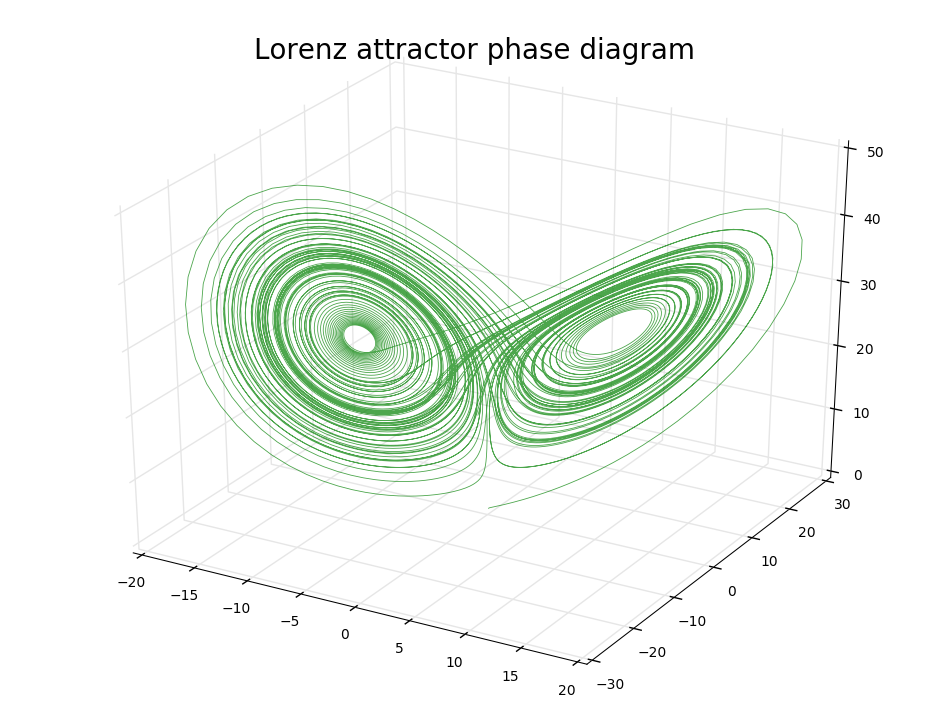
\includegraphics[scale=0.5]{1.png}
\end{center}

\begin{center}
\includegraphics[scale=0.5]{3.png}
\end{center}
\end{document}
